\documentclass[runningheads]{llncs}

\usepackage{float}
\usepackage{graphicx}
\usepackage{tikz}

\newcommand{\stargraph}[2]{\begin{tikzpicture}
	\node[circle,fill=red] at (360:0mm) (center) {Server};
    	\foreach \n in {1,...,#1}{
        		\node[circle,fill=yellow] at ({\n*360/#1}:#2cm) (n\n) {Clent \n};
        		\draw (center)--(n\n);
    }
\end{tikzpicture}}

\begin{document}
\title{Computer Networks\\ Homework 2\\ MySSH}
\author{Nistor Marian-Sergiu}
\institute{University Al. I. Cuza Iasi - Faculty of Computer Science - IIB6}

\maketitle

\begin{abstract}
This paper illustrates the architecture of the given network and the patterns, models, technologies and techniques used in order to design it.

\end{abstract}

\section{Introduction}
The project consists of a network, based on the Server-Client architecture, that behaves as a UNIX-based SSH server-clients pair. The server executes commands received from the clients and echoes the commands' results back to the requesters. An encryption mechanism will be used in order to ensure the security of the system. Each client has a corresponding shell opened on the server machine, that executes the actions requested by its associated client exclusively.

\section{Used technologies}
The main server was implemented using the concurrent TCP Server-Client model, in order to be able to process more requests at once and ensure the integrity of the data that is being sent from or towards the clients. A web HTTP-based implementation would not be viable as a stateful connection is mandatory for mantainting a certain state of the client(current execution physical location in the filesystem). The HTTP protocol is a stateless protocol.\\
The local server uses the concurrent AF\textunderscore UNIX Server-Client model, in order to skip the TCP/IP network layers, therefore being able to provide or receive data faster from and towards the main server. Its primary use is stopping the main server process. This implementation was preferred over forcing a process exit on the main server, in order to ensure that the client connections are safely closed and the used memory is released accordingly. I've also opted for this design because the idea of communicating between the terminal and the main server through a local server assures easier further development of the server.\\
The primary hashing mechanism used by the main server and the local server is SHA-256 encryption. The secondary encryption mechanism used is the Vigenere cipher, using a generic length prefix, a unique public key shared between the main server and the client and a generic length suffix. Its only use cases are when the data cannot be predicted by the other party, making SHA-256 not viable.\\
For future development, a remote desktop connection server is taken into consideration, consisting of an UDP server for desktop streaming and a TCP server for transmitting the commands(key presses and mouse clicks) towards the other party.

\section{Application architecture}

The detailed application architecture is being portrayed in the following diagram :\\

\begin{figure}[H]
\centering
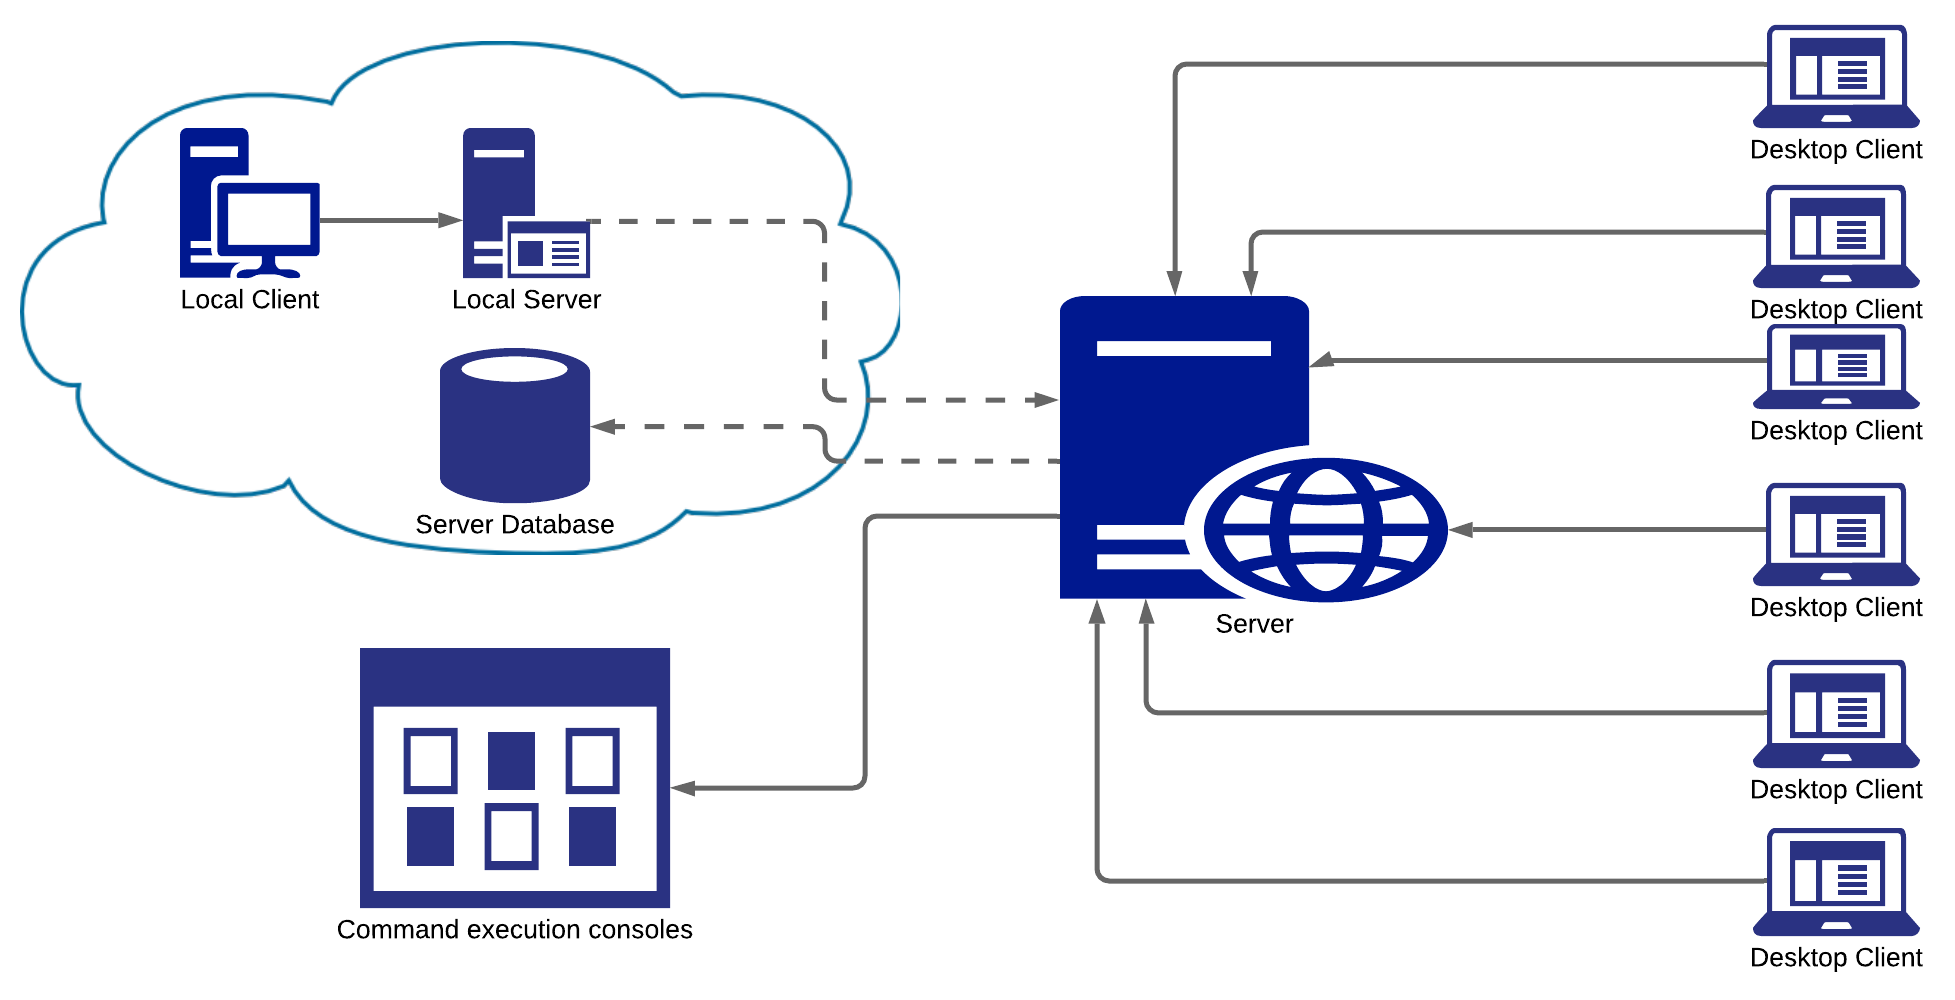
\includegraphics[width=150mm]{Network Diagram.png}
\end{figure}

A simplified graphical representation of the network, viewed from the client's perspective(therefore, without taking the idea of the \it {Cloud} into account), would be the the following star graph :\\

\stargraph {10} {4}

This raises an issue regarding the chosen design. The main server acts as a SPOF(Single Point Of Failure), as if the given node is not available, the whole network is going to be down. Though, as the idea of the project is that the commands should be executed solely on the server machine, distributed the system would result in having to abandon the original idea of the project.

\subsection{Main server transactions}
A client is uniquely identified by a tuple consisting of his IP and MAC addresses. The main server gets information from the database regarding whitelisted tuples and accepts or rejects the connection request. If the connection is accepted, it awaits a login request, containing an administrator username and password, which again are being confirmed using database information.
After the whitelisted client was logged in, his requests are being processed in a new bash console process and the responses are echoed back to the client.  Each client has a corresponding shell opened on the server machine, that executes the actions requested by its associated client exclusively. After executing the desired commands, the client can close the connection and inform the server regarding this action.\\\\

\subsection{Cloud transactions - Local server transactions}
A local server is running concurrently with the main server, awaiting commands received from a local client. The local client can stop the main server by sending a generic message through the local server.\\

\section{Implementation details}
The main server implements a TCP Server-Client architecture to ensure the consistency of exchanged data.\\
Concurrent design patterns were used for the servers(the main and local one) in order to handle multiple client connections at the same time.\\
The main server does not provide IPv6 support.\\
The local server is using a concurrent AF\textunderscore UNIX Server-Client architecture to skip the TCP/IP network layers and provide better response time from and towards the main server.\\
In the event of a forced process exit on the main server, resources are being released and clients are being disconnected. In order to achieve this, the native $\it {at\textunderscore quick\textunderscore exit}$ C++ event trigger has been used.\\
The singleton class design pattern was used to prevent the existence of several instances of the main and the local server, as only one instance should be used.

\begin{figure}[H]
\centering
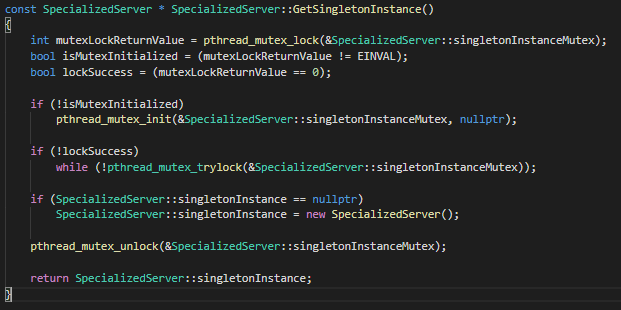
\includegraphics[width=100mm]{Singleton_Class_Design_Pattern.png}
\end{figure}
Encapsulation and inheritance(Object Oriented Design Principles) were used to enforce similarity in the behaviour of given entities. For example, both the LocalServer and the SpecializedServer classes inherit the Server class.\\
\begin{figure}[H]
\centering
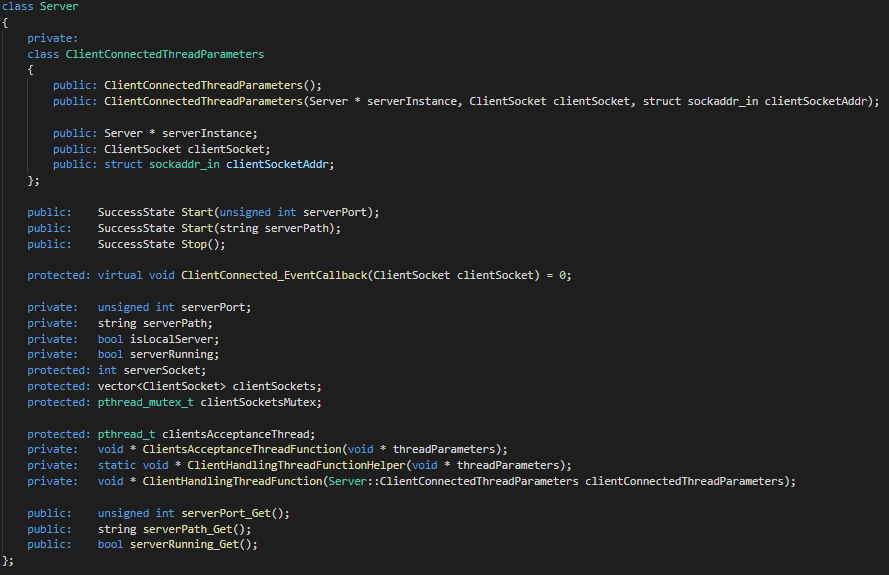
\includegraphics[width=150mm]{Server.png}
\end{figure}
\begin{figure}[H]
\centering
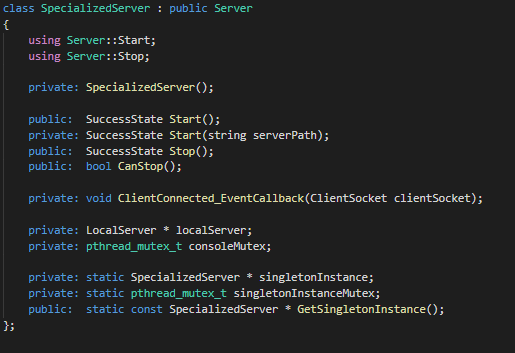
\includegraphics[width=100mm]{SpecializedServer.png}
\end{figure}
\begin{figure}[H]
\centering
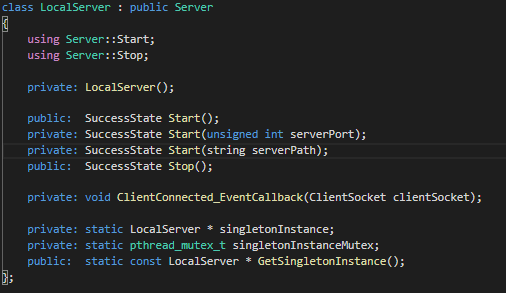
\includegraphics[width=100mm]{LocalServer.png}
\end{figure}

In order to ease further development and make the whole project a maintainable one, several functions were marked as \it {virtual}, as their implementation could vary, depending on the technologies that are being used(for example, an UI-based application wouldn't have any means of receiving input from a console).\\
The event callback functions are implemented as virtual methods on the base class, meant to be inherited by the child classes, for the same aforementioned reasons.\\

Several mutexes were used in addition to the C POSIX Threads(from the \it {pthread.h} library), to avoid memory corruption when two threads would be trying to write to a specific memory block.\\
\begin{figure}[H]
\centering
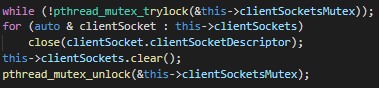
\includegraphics[width=100mm]{Mutex.png}
\end{figure}

\subsection{Centralized system}
The system is a centralized one, this model being preferred over the distributed one for this particular project. This ensures database consistency, as only one storage location is being used. However, this brings into discussion the idea that the main server becomes, therefore, a single point of failure(SPOF) in our system.

\subsection{Single point of failure(SPOF)}
The chosen network design implies a Single point of failure(SPOF) - the main server, as the system is a centralized one, having only one master node.

\subsection{Data encryption and security}

\subsubsection{SHA-256 hashing}
The primary hashing mechanism used by the main server and the local server is SHA-256 encryption. The secondary encryption mechanism used is the Vigenere cipher, using a generic length prefix, a unique public key shared between the main server and the client and a generic length suffix. Its only use cases are when the data cannot be predicted by the other party, making SHA-256 not viable. Therefore, SHA-256 hashing is used during the initial stage of the connection life-cycle, when the client IP, MAC and the administrator credentials are being sent towards the server for validation and the response is echoed back to the client. After this stage, Vigenere cipher encryption is mostly used, as the commands received from the client and their execution results are not predictable by the other party.\\
SHA-256 hashing is being implemented using the \it {openssl/sha.h} library.\\\\
The hashing function is implemented as follows :\\
\begin{figure}[H]
\centering
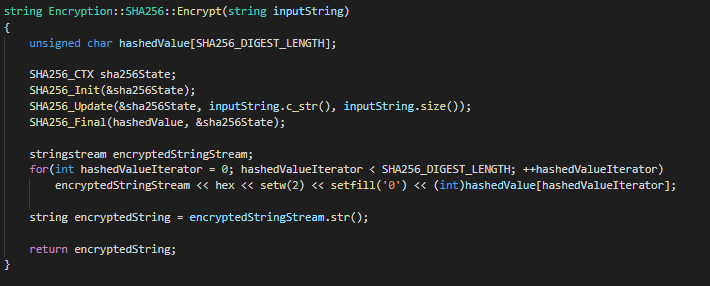
\includegraphics[width=150mm]{SHA-256_Encryption.png}
\end{figure}

The decryption function is implemented as follows :\\
\begin{figure}[H]
\centering
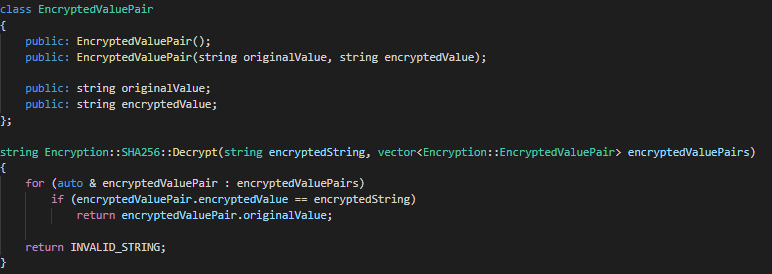
\includegraphics[width=150mm]{SHA-256_Decryption.png}
\end{figure}

\subsubsection{Vigenere encryption}
For the Vigenere encryption implementation I've opted for a custom \it {CharArray} class, because in a Vigenere-encrpyted string, the end-of-string character doesn't necessarily point towards the end of the string. Also, the custom\it {CharArray} class doesn't represent a null-terminated string.\\
\begin{figure}[H]
\centering
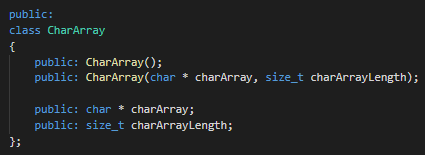
\includegraphics[width=150mm]{Vigenere_CharArray.png}
\end{figure}

The encryption function is implemented as follows :\\
\begin{figure}[H]
\centering
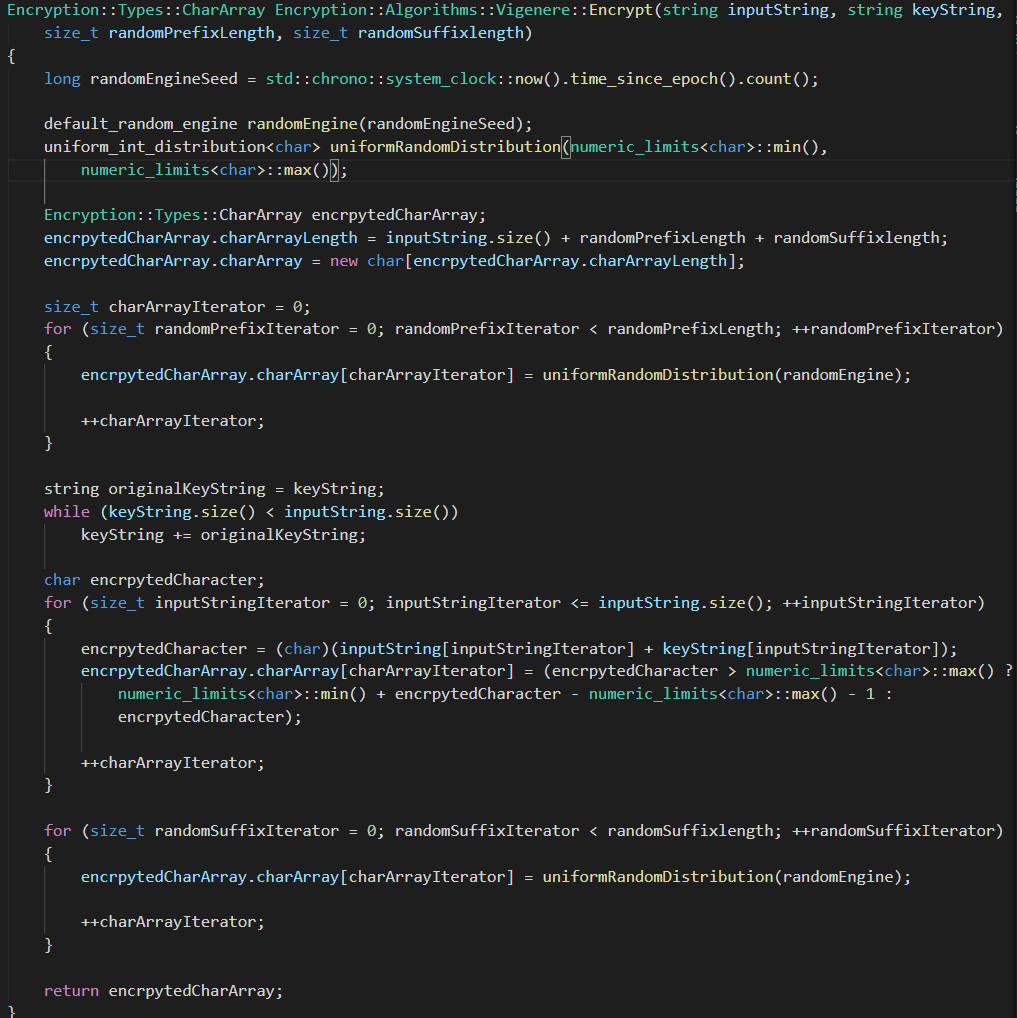
\includegraphics[width=150mm]{Vigenere_Encryption.png}
\end{figure}

The decryption function is implemented as follows :\\
\begin{figure}[H]
\centering
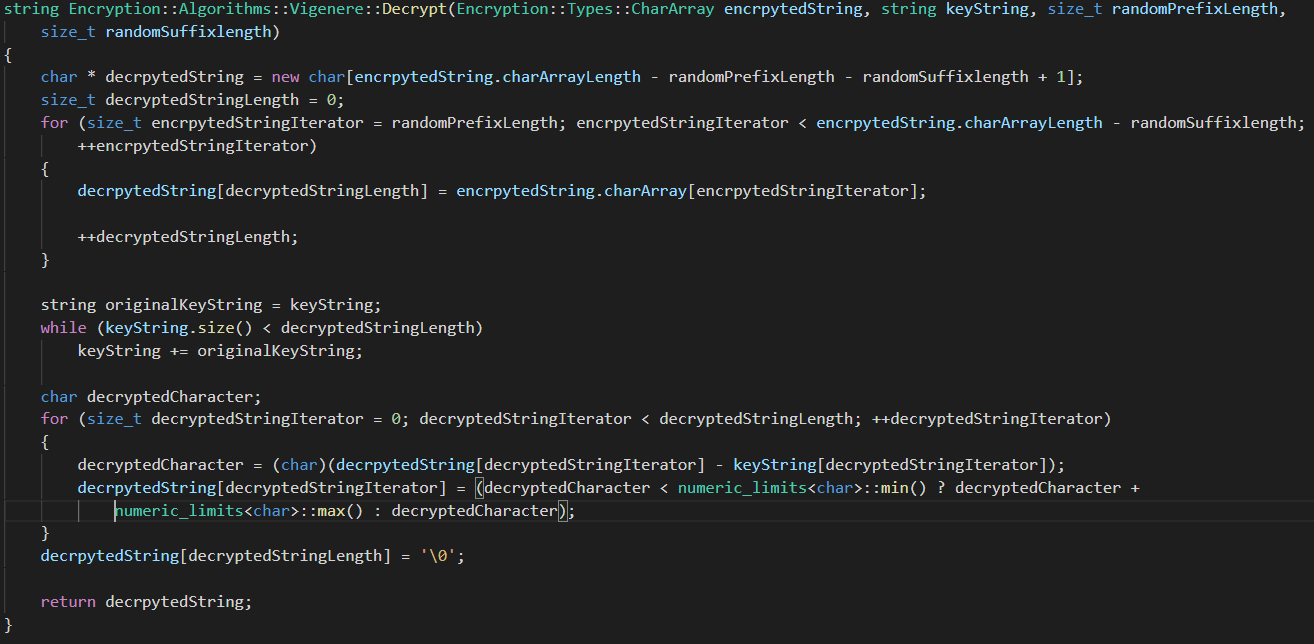
\includegraphics[width=150mm]{Vigenere_Decryption.png}
\end{figure}

\subsubsection{Prepared MySQL statements and constraints}
Prepared MySQL statements are being used as form of security against SQL Injection attacks, as such :\\
\begin{figure}[H]
\centering
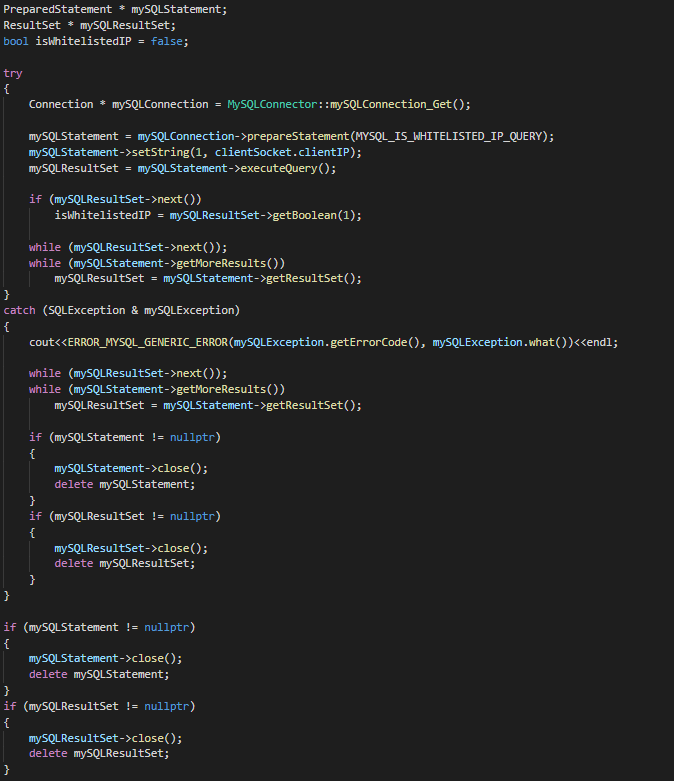
\includegraphics[width=150mm]{MySQL_Prepared_Statements.png}
\end{figure}

Database constraints were implemented using MySQL table triggers, to ensure that the fields have certain patterns.\\
\begin{figure}[H]
\centering
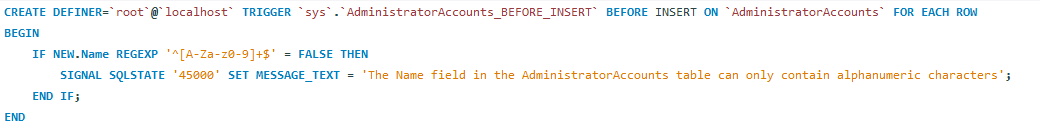
\includegraphics[width=150mm]{MySQL_Table_Triggers.png}
\end{figure}

\subsubsection{Additional security measures}
The main server cannot be started or stopped unless the requester is logged in as superuser on the server machine. The local server is being controlled only by the main server.\\
\begin{figure}[H]
\centering
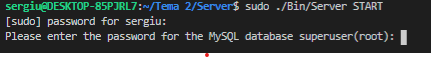
\includegraphics[width=100mm]{Superuser.png}
\end{figure}

\section{Conclusions}
The centralized system is the easier and the more viable implementation for the given project, as the client's interest would be executing commands solely on the server machine. A centralized database would also be the better fitting choice, as the data load is low, storing mostly whitelisted IP addresses, MAC addresses and administrator credentials. The main use case of the application would be sending remote controls to a server, in the context of a company. Therefore, the number of clients with the ability to connect to the server would be a low one.

\subsection{Remote desktop connection application}
The idea of a remote desktop connection application could also be taken into consideration, giving the client the possibility of connecting to the server machine, for a better user experience(UX).\\
This would bring into discussion two more servers : an unidirectional TCP server and an unidirectional UDP server. No more than one remote desktop connection should be allowed. Therefore, the TCP and UDP servers would block any other incoming connections after one has been established.\\
The TCP server would transmit the information regarding pressed keys and control triggers from the client, towards the server machine. The UDP server would send the desktop data stream towards the client.\\
The first server would use the TCP/IP protocol in order to ensure the integrity of the data sent towards the server, regarding the control triggers. This wouldn't affect the performance of the server anyhow, as the number of commands would not be a high one.\\
The second server would use the UDP/IP protocol for streaming the server's desktop, as lots of packages would have to be sent in a small amount of time. Data integrity is not crucial in this situation, while performance is a point of focus.\\

\begin{figure}[H]
\centering
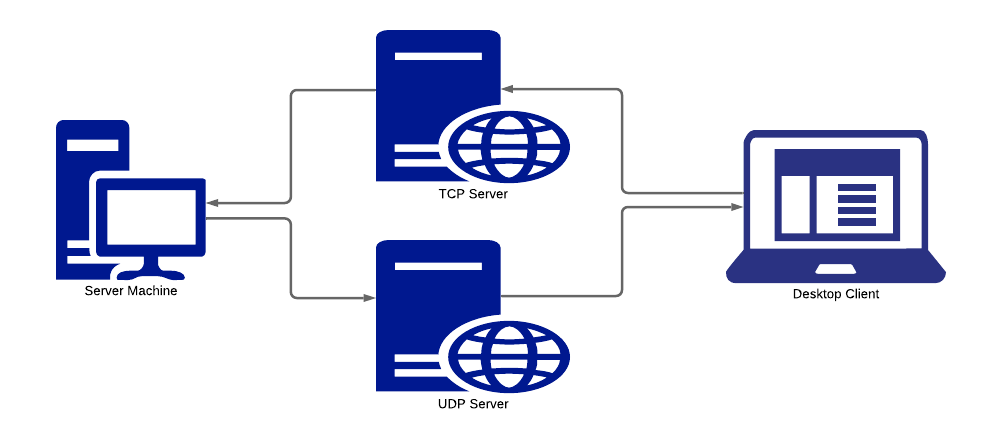
\includegraphics[width=150mm]{RDC Network Diagram.png}
\end{figure}

\begin{thebibliography}{8}

\bibitem{}
Bal, H.E., Steiner, J.G., Tanenbaum, A.S.: Programming Languages for Distributed Computing Systems, Association for Computing Machinery(ACM) (1989)
\bibitem{}
Tanenbaum, A.: Computer Networks. Prentice Hall (1981)
\bibitem{}
Computer Networks - Faculty of Computer Science \url{https://profs.info.uaic.ro/\textasciitilde computernetworks/index.php}
\bibitem{}
Wikipedia - Secure Hash Algorithms \url{https://en.wikipedia.org/wiki/Secure\textunderscore Hash\textunderscore Algorithms}
\bibitem{}
Wikipedia - SHA-2 \url{https://en.wikipedia.org/wiki/SHA-2}
\bibitem{}
Wikipedia - Vigenere cipher \url{https://en.wikipedia.org/wiki/Vigenere\textunderscore cipher}
\bibitem{}
Wikipedia - Distributed Computing \url{https://en.wikipedia.org/wiki/Distributed\textunderscore computing}
\bibitem{}
Wikipedia - Single point of failure \url{https://en.wikipedia.org/wiki/Single\textunderscore point\textunderscore of\textunderscore failure}
\bibitem{}
Wikipedia - Event-driven architecture \url{https://en.wikipedia.org/wiki/Event-driven\textunderscore architecture}
\bibitem{}
Oracle Academy - Database Design and Programming with SQL \url{https://academy.oracle.com/pages/database\textunderscore design\textunderscore course.pdf}
\bibitem{}
Peter Coad - Object-Oriented Patterns \url{https://courses.cs.washington.edu/courses/cse503/\\04sp/readings/designpattern.pdf}

\end{thebibliography}
\end{document}
